% Copyright 2004 by Till Tantau <tantau@users.sourceforge.net>.
%
% In principle, this file can be redistributed and/or modified under
% the terms of the GNU Public License, version 2.
%
% However, this file is supposed to be a template to be modified
% for your own needs. For this reason, if you use this file as a
% template and not specifically distribute it as part of a another
% package/program, I grant the extra permission to freely copy and
% modify this file as you see fit and even to delete this copyright
% notice. 

\documentclass{beamer}

\usepackage{kotex}
\usepackage{graphicx,psfrag,amsfonts,amsmath,amssymb}
\usepackage{multicol}

% code block option
\usepackage{listings}
\usepackage{xcolor}

\definecolor{codegreen}{rgb}{0,0.6,0}
\definecolor{codegray}{rgb}{0.5,0.5,0.5}
\definecolor{codepurple}{rgb}{0.58,0,0.82}
\definecolor{backcolour}{rgb}{0.95,0.95,0.92}

\lstdefinestyle{mystyle}{
	backgroundcolor=\color{backcolour},   
	commentstyle=\color{codegreen},
	keywordstyle=\color{magenta},
	numberstyle=\tiny\color{codegray},
	stringstyle=\color{codepurple},
	basicstyle=\ttfamily\footnotesize,
	breakatwhitespace=false,         
	breaklines=true,                 
	captionpos=b,                    
	keepspaces=true,                 
	numbers=left,                    
	numbersep=5pt,                  
	showspaces=false,                
	showstringspaces=false,
	showtabs=false,                  
	tabsize=2
}

\lstset{style=mystyle}

% There are many different themes available for Beamer. A comprehensive
% list with examples is given here:
% http://deic.uab.es/~iblanes/beamer_gallery/index_by_theme.html
% You can uncomment the themes below if you would like to use a different
% one:
%\usetheme{Dresden}
%\usetheme{AnnArbor}
%\usetheme{Antibes}
%\usetheme{Bergen}
%\usetheme{Berkeley}
\usetheme{Berlin}
%\usetheme{Boadilla}
%\usetheme{boxes}
%\usetheme{CambridgeUS}
%\usetheme{Copenhagen}
%\usetheme{Darmstadt}
%\usetheme{default}
%\usetheme{Frankfurt}
%\usetheme{Goettingen}
%\usetheme{Hannover}
%\usetheme{Ilmenau}
%\usetheme{JuanLesPins}
%\usetheme{Luebeck}
%\usetheme{Madrid}
%\usetheme{Malmoe}
%\usetheme{Marburg}
%\usetheme{Montpellier}
%\usetheme{PaloAlto}
%\usetheme{Pittsburgh}
%\usetheme{Rochester}
%\usetheme{Singapore}
%\usetheme{Szeged}
%\usetheme{Warsaw}

\usecolortheme{lily}
\usefonttheme[onlymath]{serif}	% 수식 설정!!

\title{Introduction to \LaTeX}
%\date{\today}
\date[Short Occasion]{Febrary 5, 2020}
\author{Hyunsung Kim}
\institute[Dept. of Statistics]
	{Department of Statistics\\
	Chung-Ang University}

% A subtitle is optional and this may be deleted
%\subtitle{소제목}

%\author{F.~Author\inst{1} \and S.~Another\inst{2}}
% - Give the names in the same order as the appear in the paper.
% - Use the \inst{?} command only if the authors have different
%   affiliation.

%\institute[Universities of Somewhere and Elsewhere] % (optional, but mostly needed)
%{
%  \inst{1}%
%  Department of Computer Science\\
%  University of Somewhere
%  \and
%  \inst{2}%
%  Department of Theoretical Philosophy\\
%  University of Elsewhere}
% - Use the \inst command only if there are several affiliations.
% - Keep it simple, no one is interested in your street address.

%\date{Conference Name, 2013}
% - Either use conference name or its abbreviation.
% - Not really informative to the audience, more for people (including
%   yourself) who are reading the slides online

\subject{Introduction to \LaTeX}
% This is only inserted into the PDF information catalog. Can be left
% out. 

% If you have a file called "university-logo-filename.xxx", where xxx
% is a graphic format that can be processed by latex or pdflatex,
% resp., then you can add a logo as follows:

% \pgfdeclareimage[height=0.5cm]{university-logo}{university-logo-filename}
% \logo{\pgfuseimage{university-logo}}

% Delete this, if you do not want the table of contents to pop up at
% the beginning of each subsection:
\AtBeginSubsection[]
{
  \begin{frame}<beamer>{Outline}
    \tableofcontents[currentsection,currentsubsection]
  \end{frame}
}

% Let's get started
\begin{document}

\begin{frame}
  \titlepage
\end{frame}

\begin{frame}{Outline}
  \tableofcontents
  % You might wish to add the option [pausesections]
\end{frame}

% Section and subsections will appear in the presentation overview
% and table of contents.
\section{Useful methods}

\subsection{\texttt{xtable} package}

\begin{frame}{\texttt{xtable} package}
  \begin{itemize}
  	\item {
	    \texttt{R}의 dataframe or matrix 형태를 \textrm{\LaTeX} 코드로 변환시켜주는 package
	}
	\item {
		print되는 output을 그대로 복사해서 사용하면 됨
	}
  \end{itemize}
\end{frame}

\begin{frame}{\texttt{xtable} package}
	\begin{figure}[h] %%% t: top, b: bottom, h: here
		\begin{center}
			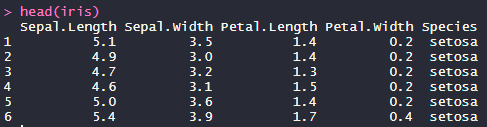
\includegraphics[width=0.9\linewidth]{img/xtable1.png}
		\end{center}
		\caption{The sample dataframe object}
		\label{fig:long}
		\label{fig:onecol}
	\end{figure}
\end{frame}

\begin{frame}{\texttt{xtable} package}
	\begin{figure}[h] %%% t: top, b: bottom, h: here
		\begin{center}
			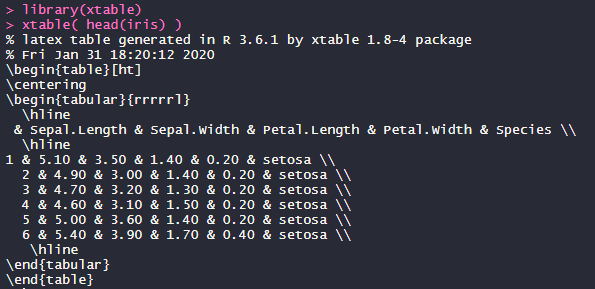
\includegraphics[width=0.9\linewidth]{img/xtable2.png}
		\end{center}
		\caption{Output of \texttt{xtable} function}
		\label{fig:long}
		\label{fig:onecol}
	\end{figure}
\end{frame}

\begin{frame}{\texttt{xtable} package}
	\begin{table}[ht]
		\centering
		\tiny
		\begin{tabular}{rrrrrl}
			\hline
			& Sepal.Length & Sepal.Width & Petal.Length & Petal.Width & Species \\ 
			\hline
			1 & 5.10 & 3.50 & 1.40 & 0.20 & setosa \\ 
			2 & 4.90 & 3.00 & 1.40 & 0.20 & setosa \\ 
			3 & 4.70 & 3.20 & 1.30 & 0.20 & setosa \\ 
			4 & 4.60 & 3.10 & 1.50 & 0.20 & setosa \\ 
			5 & 5.00 & 3.60 & 1.40 & 0.20 & setosa \\ 
			6 & 5.40 & 3.90 & 1.70 & 0.40 & setosa \\ 
			\hline
		\end{tabular}
	\caption{The table using output of \texttt{xtable} function}
	\end{table}
\end{frame}


\subsection{User defined command}

\begin{frame}{User defined command}
	\begin{itemize}
		\item {
			수식 작성시 반복해서 사용하게 되는 코드가 생김(bold체 등)
		}
		\item {
			\textrm{\LaTeX} 파일 상단에 축약해놓은 명령어를 지정해 놓고 사용하면 매우 편리!
		}
	\end{itemize}
\end{frame}

\begin{frame}[fragile]{Before using user defined command}
	$$ \mathbf{B}_i\boldsymbol{\Theta}\mathbf{D}\boldsymbol{\Theta}^T\mathbf{B}^T_i $$
	
	\begin{lstlisting}
	% Don't use user defined command
	$$ \mathbf{B}_i \boldsymbol{\Theta} \mathbf{D} \boldsymbol{\Theta}^T \mathbf{B}^T_i $$  \end{lstlisting}
\end{frame}

\begin{frame}[fragile]{User defined command}
	\begin{lstlisting}
	\def \bY { \mathbf{Y} }
	\def \bB { \mathbf{B} }
	\def \bI { \mathbf{I} }
	\def \bD { \mathbf{D} }
	\def \bbeta { \boldsymbol{\beta} }
	\def \btheta { \boldsymbol{\theta} }
	\def \bTheta { \boldsymbol{\Theta} }
	\def \balpha { \boldsymbol{\alpha} }  \end{lstlisting}
\end{frame}

\begin{frame}[fragile]{After using user defined command}
	\def \bY {\mathbf{Y}}
	\def \bB {\mathbf{B}}
	\def \bI {\mathbf{I}}
	\def \bD {\mathbf{D}}
	\def \bbeta {\boldsymbol{\beta}}
	\def \btheta {\boldsymbol{\theta}}
	\def \bTheta {\boldsymbol{\Theta}}
	\def \balpha {\boldsymbol{\alpha}}
	
	$$ \bB_i\bTheta\bD\bTheta^T\bB^T_i $$
	
	\begin{lstlisting}
	% Use user defined command
	$$ \bB_i \bTheta \bD \bTheta^T \bB^T_i $$ \end{lstlisting}
\end{frame}


\subsection{Code block}

\begin{frame}{Code block}
	\begin{itemize}
		\item {
			간혹 과제 제출할 때, 코드를 같이 제출하게 되는 강의를 들을 때 유용(통계계산론, 데이터마이닝 등등)
		}
		\item {
			단순히 코드 복사해서 붙여넣는 것보다는 나름 깔끔하게 정리 가능
		}
		\item {
			설명은 링크로 대체 $\Rightarrow$ \url{https://www.overleaf.com/learn/latex/Code_listing}
		}
	\end{itemize}
\end{frame}

\begin{frame}{Cross-covariance and cross-correlation functions}{Cantour plots of correlation functions}
	\begin{multicols}{2}
		\begin{figure}[h] %%% t: top, b: bottom, h: here
			\begin{center}
				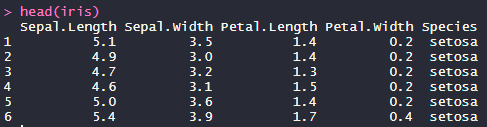
\includegraphics[width=0.9\linewidth]{img/xtable1.png}
			\end{center}
			%\caption{Sampling two normal mixture(histogram) VS True normal mixture(red line)}
			\label{fig:long}
			\label{fig:onecol}
		\end{figure}
		\begin{figure}[h] %%% t: top, b: bottom, h: here
			\begin{center}
				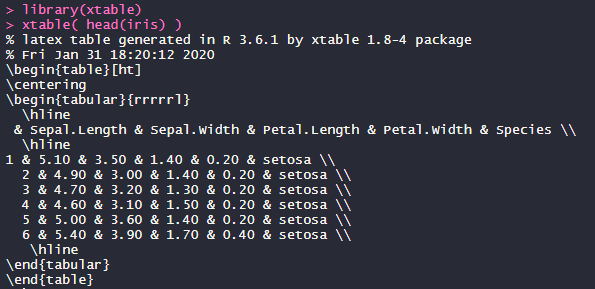
\includegraphics[width=0.9\linewidth]{img/xtable2.png}
			\end{center}
			%\caption{Sampling two normal mixture(histogram) VS True normal mixture(red line)}
			\label{fig:long}
			\label{fig:onecol}
		\end{figure}
	\end{multicols}
\end{frame}


%\appendix
\section*{Appendix}
\subsection<presentation>*{Reference}

\begin{frame}
  \frametitle<presentation>{Reference}
    
  \begin{thebibliography}{10}
    
  \beamertemplatebookbibitems
  % Start with overview books.

	\bibitem{Author1990}
		J.O. Ramsay, B.W. Silverman.
		\newblock {\em Functional Data Analysis 2nd edition}.
		\newblock Springer, 2005.
 
    
%  \beamertemplatearticlebibitems
%  % Followed by interesting articles. Keep the list short. 
%
%  \bibitem{Someone2000}
%    S.~Someone.
%    \newblock On this and that.
%    \newblock {\em Journal of This and That}, 2(1):50--100,
%    2000.
  \end{thebibliography}
\end{frame}
\section*{Appendix}

% All of the following is optional and typically not needed. 
%\appendix
%\section<presentation>*{\appendixname}
%\subsection<presentation>*{For Further Reading}
%
%\begin{frame}[allowframebreaks]
%  \frametitle<presentation>{For Further Reading}
%    
%  \begin{thebibliography}{10}
%    
%  \beamertemplatebookbibitems
%  % Start with overview books.
%
%  \bibitem{Author1990}
%    A.~Author.
%    \newblock {\em Handbook of Everything}.
%    \newblock Some Press, 1990.
% 
%    
%  \beamertemplatearticlebibitems
%  % Followed by interesting articles. Keep the list short. 
%
%  \bibitem{Someone2000}
%    S.~Someone.
%    \newblock On this and that.
%    \newblock {\em Journal of This and That}, 2(1):50--100,
%    2000.
%  \end{thebibliography}
%\end{frame}

\end{document}


